% Provenance (never printed): see sources/outline_sources.md (Year 3:
% facies analysis, depositional models, Walther's law, well logs). Brief:
% sources/book5/BRIEFS.md, ch. 17. Curves from figdata/bachelor-3/well_logs.py
% (unit tops from figdata/shared/region.py). Exercise and problem values in
% the Book 5 scratch calculator calc/ch17.py. The well Varden-2, its logs and
% the channel architecture of its sandstone are invented.
\chapter{Facies Models}\label{ch:b3:facies-models}

A core from a well a kilometre deep: a metre of coarse sand with
cross-beds resting on a sharp base, fining upward into silt with the traces
of roots, then sand again on another sharp base. The geologist reads a river
that wandered across its plain, though no river runs there now. The reading
rests on two tools: a set of models, each a summary of many modern and
ancient examples of one environment, and a law that turns a vertical
succession of beds into a map of neighbouring environments.

\begin{recall}
Sedimentary facies, depositional environment, bedforms, cross-bedding,
deltas of the three kinds, turbidity currents, turbidites and graded beds are
in the Year 1 volume, in its chapter on clastic sediments and their
environments; the carbonate factory, reefs and carbonate platforms in its
chapter on carbonate, siliceous and evaporite sediments; the borehole log and
the correlation of logs in its chapter on cross-sections. Porosity and
permeability are in the school books. \omterm{def:b3:sequence-stratigraphy:parasequence}{Parasequences}, \omterm{def:b3:sequence-stratigraphy:parasequence}{flooding surfaces} and
\omterm{def:b3:sequence-stratigraphy:tract}{systems tracts} are in Chapter~\ref{ch:b3:sequence-stratigraphy}. Waves on
deep water, whose motion fades with depth, are in the physics books.
\end{recall}

\section{Facies, successions and Walther's law}\label{sec:b3:facies-models:walther}

A sedimentary facies is described from what can be seen in a core or a
cliff: grain size, sorting, structures, fossils, colour. A single facies is
rarely diagnostic: cross-bedded sand forms in rivers, on beaches, in tidal
channels and in deserts. What identifies an environment is the company a
facies keeps and the order in which facies follow one another.

\begin{definition}[Facies association and facies succession]\label{def:b3:facies-models:association}
A \emph{facies association}\index{facies association} is a group of facies
that occur together and were deposited in one environment, such as channel
sand, levee silt and floodplain mud with roots. A \emph{facies
succession}\index{facies succession} is a vertical sequence of facies in
which some property changes progressively upward; in a \emph{fining-upward
succession}\index{fining-upward succession} the grain size decreases upward,
in a \emph{coarsening-upward succession}\index{coarsening-upward succession}
it increases.
\end{definition}

\begin{definition}[Facies model]\label{def:b3:facies-models:model}
A \emph{facies model}\index{facies model} is a general summary of a
depositional environment, distilled from many modern and ancient examples: the
facies it produces, their geometry, their lateral relations and the
successions they build. It serves as a norm to compare a new example with, a
guide for further observation, a predictor in new situations, and a basis for
interpreting the environment.
\end{definition}

The bridge between the lateral and the vertical is a law. Neighbouring
environments lie side by side at any moment: the beach next to the
\omterm{def:b3:facies-models:shoreface}{shoreface}, the \omterm{def:b3:facies-models:shoreface}{shoreface} next to the offshore mud. When the shoreline moves,
each environment comes to lie over its neighbour.

\begin{theorem}[Walther's law]\label{thm:b3:facies-models:walther}
In a conformable succession, without a significant break in deposition or an
erosional surface, facies that lie directly above one another were deposited
in environments that lay side by side at the time.
\end{theorem}

\begin{proof}
Consider belts of environments, each a strip parallel to the shoreline, that
migrate together across the basin while the floor subsides or the sea level
rises. At a fixed place the belts pass over one after the other, in the order
in which they lie side by side, and each leaves its deposit on top of the
deposit of the belt that preceded it. If deposition is continuous, the
vertical order of the deposits is therefore the lateral order of the belts.
A break or an erosion surface interrupts the argument: the belts that passed
during the gap left nothing, or their deposits were removed, and facies from
non-adjacent environments come into contact.
\end{proof}

\begin{omfigure}
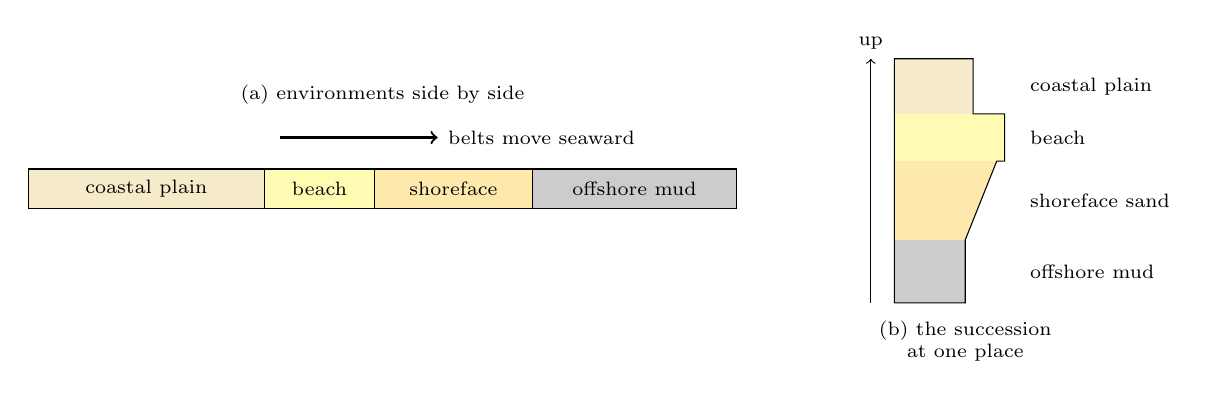
\begin{tikzpicture}[font=\scriptsize, x=1cm, y=1cm]
% environments side by side, with a shoreline that moves seaward
\fill[yellow!35!brown!25] (0,0) rectangle (3,0.5);
\fill[yellow!30] (3,0) rectangle (4.4,0.5);
\fill[yellow!50!orange!30] (4.4,0) rectangle (6.4,0.5);
\fill[black!20] (6.4,0) rectangle (9,0.5);
\draw (0,0) rectangle (9,0.5);
\foreach \x in {3,4.4,6.4} {\draw (\x,0) -- (\x,0.5);}
\node at (1.5,0.25) {coastal plain};
\node at (3.7,0.25) {beach};
\node at (5.4,0.25) {shoreface};
\node at (7.7,0.25) {offshore mud};
\draw[->, thick] (3.2,0.9) -- (5.2,0.9) node[right] {belts move seaward};
\node[anchor=south] at (4.5,1.2) {(a) environments side by side};
% vertical succession at a place
\begin{scope}[xshift=11cm, yshift=-1.2cm]
\fill[black!20] (0,0) rectangle (0.9,0.8);
\fill[yellow!50!orange!30] (0,0.8) -- (0.9,0.8) -- (1.3,1.8) -- (0,1.8) -- cycle;
\fill[yellow!30] (0,1.8) rectangle (1.4,2.4);
\fill[yellow!35!brown!25] (0,2.4) rectangle (1.0,3.1);
\draw (0,0) -- (0.9,0) -- (0.9,0.8) -- (1.3,1.8) -- (1.4,1.8) -- (1.4,2.4) -- (1.0,2.4) -- (1.0,3.1) -- (0,3.1) -- cycle;
\node[anchor=west] at (1.6,0.4) {offshore mud};
\node[anchor=west] at (1.6,1.3) {shoreface sand};
\node[anchor=west] at (1.6,2.1) {beach};
\node[anchor=west] at (1.6,2.75) {coastal plain};
\draw[->] (-0.3,0) -- (-0.3,3.1) node[above] {up};
\node[anchor=north, align=center] at (0.9,-0.1) {(b) the succession\\ at one place};
\end{scope}
\end{tikzpicture}

\par\smallskip{\small Walther's law. (a) Environments lie side by side along
a profile; (b) as the belts move seaward, one place receives offshore mud,
then \omterm{def:b3:facies-models:shoreface}{shoreface} sand, beach sand and coastal-plain deposits: a
\omterm{def:b3:facies-models:association}{coarsening-upward succession} in the order of the belts (width in the log
means coarser grain).}\label{fig:b3:facies-models:walther}
\end{omfigure}

The law works both ways. A regression stacks the belts in their seaward order
upward, a transgression in the reverse order; and a vertical succession read in
a core gives the map of the neighbouring environments at the time. It fails
exactly where Chapter~\ref{ch:b3:sequence-stratigraphy} puts its key surfaces:
across a \omterm{def:b3:sequence-stratigraphy:sequence}{sequence boundary}, where exposure and erosion bring river sand onto
shelf mud, and across a \omterm{def:b3:sequence-stratigraphy:parasequence}{flooding surface}, where offshore mud lies directly on
the coastal plain.

\section{Rivers}\label{sec:b3:facies-models:rivers}

\begin{definition}[Braided and meandering rivers]\label{def:b3:facies-models:rivers}
A \emph{braided river}\index{braided river} flows in several shallow
channels that divide and rejoin around bars, on a steep plain with abundant
coarse load and variable discharge. A \emph{meandering river}\index{meandering
river} flows in a single sinuous channel on a gentler plain, carrying more
fine sediment; it migrates by eroding the outer bank of each bend and
depositing on the inner one. The deposit on the inner bank is a \emph{point
bar}\index{point bar}. \emph{Avulsion}\index{avulsion} is the abandonment of
a channel for a new course across the floodplain, usually after a flood
breaches a levee.
\end{definition}

A \omterm{def:b3:facies-models:rivers}{point bar} grows sideways as the bend migrates, so at any place it records
the cross-section of the channel from bottom to top: a lag of the coarsest
clasts on an erosional base, cross-bedded sand from the dunes of the deep
channel, finer sand with ripples from the shallow top of the bar, then the
silt and mud of the floodplain with roots and soils. By Walther's law this
\omterm{def:b3:facies-models:association}{fining-upward succession}, a few metres thick, has the thickness of the
channel's depth. A \omterm{def:b3:facies-models:rivers}{braided river} leaves stacked sheets of cross-bedded sand
and gravel with little mud, whose grain size hardly changes upward; its fines
are carried away. \omterm{def:b3:facies-models:rivers}{Avulsion} moves the channel belt across the plain, so that
channel bodies stack at random among floodplain muds, separated by sharp
erosional bases.

\begin{omfigure}
\begin{tikzpicture}[font=\scriptsize, x=1cm, y=1cm]
% (a) braided plan
\begin{scope}
\fill[yellow!35!brown!20] (0,0) rectangle (4.6,2.4);
\draw[omDef!60, line width=1.6pt] (0,1.2) .. controls (0.8,1.6) and (1.4,0.6) .. (2.3,1.0) .. controls (3.0,1.3) and (3.6,0.7) .. (4.6,1.0);
\draw[omDef!60, line width=1.6pt] (0,1.2) .. controls (0.8,0.8) and (1.6,1.9) .. (2.4,1.6) .. controls (3.2,1.3) and (3.8,1.9) .. (4.6,1.6);
\draw[omDef!60, line width=1.2pt] (1.2,1.25) .. controls (1.8,1.5) and (2.6,1.2) .. (3.3,1.35);
\fill[yellow!45] (1.5,1.15) ellipse (0.35 and 0.12);
\fill[yellow!45] (3.0,1.25) ellipse (0.4 and 0.12);
\node[anchor=south] at (2.3,2.45) {(a) braided};
\end{scope}
% (b) meandering plan
\begin{scope}[xshift=5.4cm]
\fill[green!30!black!12] (0,0) rectangle (4.6,2.4);
\draw[omDef!60, line width=2pt] (0,1.2) .. controls (0.6,2.2) and (1.4,2.2) .. (1.6,1.2) .. controls (1.8,0.2) and (2.8,0.2) .. (3.0,1.2) .. controls (3.2,2.2) and (4.0,2.2) .. (4.6,1.2);
\fill[yellow!45] (0.8,1.45) ellipse (0.3 and 0.2);
\fill[yellow!45] (2.3,0.95) ellipse (0.3 and 0.2);
\fill[yellow!45] (3.8,1.45) ellipse (0.3 and 0.2);
\node at (2.3,0.95) {pb};
\draw[omDef!40, line width=1pt, densely dashed] (0.4,0.2) .. controls (1.0,0.7) and (1.6,0.4) .. (2.0,0.1);
\node[anchor=west, font=\tiny] at (2.6,2.15) {floodplain};
\node[anchor=south] at (2.3,2.45) {(b) meandering};
\end{scope}
% logs
\begin{scope}[xshift=10.8cm]
\fill[yellow!45] (0,0) -- (1.2,0) -- (1.2,2.0) -- (0,2.0) -- cycle;
\draw (0,0) -- (1.2,0) -- (1.15,0.6) -- (1.2,0.65) -- (1.1,1.3) -- (1.2,1.35) -- (1.15,2.0) -- (0,2.0) -- cycle;
\node[anchor=north] at (0.6,-0.05) {braided};
\end{scope}
\begin{scope}[xshift=12.6cm]
\fill[yellow!45] (0,0) -- (1.2,0) -- (1.1,0.9) -- (0.45,1.6) -- (0,1.6) -- cycle;
\fill[green!30!black!15] (0,1.6) rectangle (0.3,2.2);
\draw (0,0) -- (1.2,0) -- (1.1,0.9) -- (0.45,1.6) -- (0.3,1.6) -- (0.3,2.2) -- (0,2.2) -- cycle;
\draw[decorate, decoration={snake, amplitude=0.4mm, segment length=1.5mm}] (0,0) -- (1.2,0);
\node[anchor=north] at (0.6,-0.05) {point bar};
\node[anchor=west, font=\tiny] at (0.35,1.9) {roots};
\end{scope}
\end{tikzpicture}

\par\smallskip{\small (a) A \omterm{def:b3:facies-models:rivers}{braided river}: several channels around bars of
sand and gravel. (b) A \omterm{def:b3:facies-models:rivers}{meandering river}: one sinuous channel, \omterm{def:b3:facies-models:rivers}{point bars} (pb)
on the inner banks, an abandoned course (dashed) left by \omterm{def:b3:facies-models:rivers}{avulsion}. Right:
grain-size logs of the deposits (width means coarser): stacked sand sheets
with little change upward for the \omterm{def:b3:facies-models:rivers}{braided river}, a sharp-based \omterm{def:b3:facies-models:association}{fining-upward
succession} capped by rooted floodplain mud for the \omterm{def:b3:facies-models:rivers}{point
bar}.}\label{fig:b3:facies-models:rivers}
\end{omfigure}

\section{Shorelines, deltas and shelves}\label{sec:b3:facies-models:shelves}

The deltas of the Year 1 volume, dominated by rivers, waves or tides, all
build out by the same mechanism: the mouth deposits its load where the
current slows, and the delta front progrades over its own prodelta muds. A
prograding delta front or \omterm{def:b3:facies-models:shoreface}{shoreface} leaves, by Walther's law, a
\omterm{def:b3:facies-models:association}{coarsening-upward succession}: offshore mud, interbedded mud and storm sand,
\omterm{def:b3:facies-models:shoreface}{shoreface} sand, beach. Each \omterm{def:b3:sequence-stratigraphy:parasequence}{parasequence} of the previous chapter is one such
succession.

\begin{definition}[Shoreface and wave bases]\label{def:b3:facies-models:shoreface}
The \emph{shoreface}\index{shoreface} is the sloping zone seaward of the
beach where waves continually rework the sea floor. Its base is the
\emph{fair-weather wave base}\index{fair-weather wave base}, the depth below
which ordinary waves no longer move the bottom sediment. The \emph{storm wave
base}\index{storm wave base} is the deeper limit reached by storm waves;
between the two, mud settles in calm weather and is reworked into sand beds
during storms. Below the storm wave base the floor is undisturbed by waves.
\end{definition}

\begin{omfigure}
\begin{tikzpicture}[font=\scriptsize, x=1cm, y=1.6cm]
\fill[omSea!60] (0,2.2) -- (13,2.2) -- (13,0.2) -- (5.5,0.9) -- (2.0,1.9) -- (0.6,2.2) -- cycle;
\fill[yellow!40] (0,2.4) -- (0.6,2.2) -- (2.0,1.9) -- (5.5,0.9) -- (5.5,0.0) -- (0,0.0) -- cycle;
\fill[black!18] (5.5,0.9) -- (13,0.2) -- (13,0) -- (5.5,0) -- cycle;
\draw[thick] (0,2.4) -- (0.6,2.2) -- (2.0,1.9) -- (5.5,0.9) -- (13,0.2);
\draw[omDef] (0,2.2) -- (13,2.2);
\draw[omDef, densely dashed] (1.6,1.97) -- (13,1.97);
\draw[omDef, densely dashed] (5.5,0.9) -- (13,0.9);
\node[omDef, anchor=north west] at (9.3,1.95) {fair-weather wave base};
\node[omDef, anchor=north west] at (9.3,0.88) {storm wave base};
\node[anchor=south] at (0.5,2.42) {beach};
\node at (1.8,1.35) {shoreface};
\node at (4.3,0.45) {offshore transition};
\node at (9.0,0.15) {offshore mud};
\node[align=center] at (7.4,1.45) {storm sand beds,\\ hummocky cross-stratification};
\end{tikzpicture}

\par\smallskip{\small A wave-dominated shoreline profile (schematic, vertical
scale much exaggerated). Above the \omterm{def:b3:facies-models:shoreface}{fair-weather wave base} the \omterm{def:b3:facies-models:shoreface}{shoreface} sand
is reworked every day; between the two wave bases mud alternates with
storm-deposited sand beds; below the \omterm{def:b3:facies-models:shoreface}{storm wave base} mud
accumulates.}\label{fig:b3:facies-models:shoreface}
\end{omfigure}

The orbital motion of a wave on deep water fades as $e^{-2\pi z/\lambda}$
with depth $z$, for a wavelength $\lambda$: at half a wavelength it keeps
\qty{4}{\percent} of its surface amplitude, which sets the scale of a wave
base. Buoy records of over two million wave spectra from the Caribbean, the
Gulf of Mexico and the western Atlantic give modal wavelengths of about
\qty{75}{m} in the sheltered seas and about \qty{110}{m} on the open margin,
and show that, averaged over weeks to years, wavelengths do not split into a
fair-weather class and a storm class: the chance that a wave stirs the bottom
rises steadily as the water shallows. The two wave bases remain useful words
for zones of a profile, not sharp depths.
% ledger: losspeters10:wavebase

\begin{definition}[Hummocky cross-stratification]\label{def:b3:facies-models:hcs}
\emph{Hummocky cross-stratification}\index{hummocky cross-stratification} is
a stratification of fine sand in gently curved laminae, concave-up
(swales) and convex-up (hummocks), that cut one another at low angles and
thicken and thin laterally, over wavelengths of a metre to several metres. It
is formed by the oscillating and combined flows of storm waves, between the
fair-weather and the \omterm{def:b3:facies-models:shoreface}{storm wave base}.
\end{definition}

\begin{inthefield}[Storm beds on a Silurian shelf]
\begin{minipage}[t]{0.42\linewidth}\vspace{0pt}
In the Arisaig Formation of Nova Scotia, layers of fine sandstone separate
darker mudstone. Geologists who studied such beds recognise the low, curved,
intersecting laminae of \omterm{def:b3:facies-models:hcs}{hummocky cross-stratification}: each bed records a
storm that stirred the shelf below the reach of everyday waves, and the mud
around it the long calm between storms.
\end{minipage}\hfill
\begin{minipage}[t]{0.54\linewidth}\vspace{0pt}
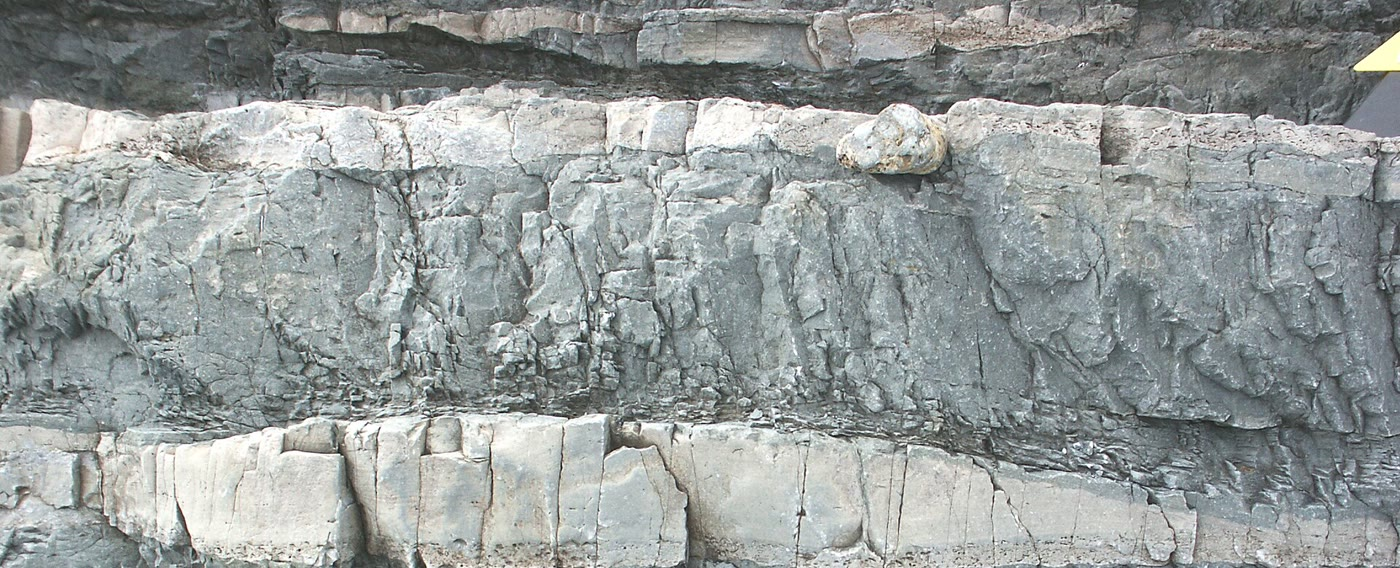
\includegraphics[width=\linewidth]{images/book5/b3-hummocky-cross-stratification.jpg}

{\scriptsize \omterm{def:b3:facies-models:hcs}{Hummocky cross-stratification} in the Arisaig Formation
(Silurian), near Arisaig, Nova Scotia. Photo Michael C. Rygel, CC BY-SA 3.0
(cropped).}
\end{minipage}
\end{inthefield}
% ledger: photo:b3-hcs

Where tides dominate, the facies change: flood and ebb currents build
cross-beds that face in opposite directions, mud drapes settle at each slack
water, and the thickness of the bundles between drapes waxes and wanes with
the cycle of spring and neap tides. Tidal channels, flats and sand ridges
have their own models, built the same way.

\section{Deep water}\label{sec:b3:facies-models:deep}

A turbidity current that slows deposits its load in the order of settling:
the coarsest grains first, the finest last. A complete turbidite bed shows
this order as five divisions.

\begin{definition}[Bouma sequence]\label{def:b3:facies-models:bouma}
The \emph{Bouma sequence}\index{Bouma sequence} is the ideal succession of
divisions in a turbidite bed, from base to top: Ta, massive or graded sand on
an erosional base with flute and tool marks; Tb, parallel-laminated sand; Tc,
ripple cross-laminated and convolute fine sand; Td, parallel-laminated silt;
Te, mud, partly from the turbidity current and partly from the slow settling
between flows.
\end{definition}

Few beds show all five: near the source the current is fast and leaves thick
Ta divisions with the upper ones eroded by the next flow; far from it only
the finer divisions, Tc to Te, arrive. The sequence thus records the
waning of one flow, and the change of the beds along the fan the waning of
the flows with distance.

\begin{definition}[Submarine fan]\label{def:b3:facies-models:fan}
A \emph{submarine fan}\index{submarine fan} is a cone of sediment at the foot
of a continental slope, fed by a canyon: an upper fan with a main channel
between levées, a middle fan of distributary channels ending in sand lobes,
and a lower fan of thin turbidites passing into basin-floor mud.
\end{definition}

Along the margin, deep currents driven by the ocean's circulation rework the
fine sediment of the slope into contourites, mounds and drifts of
bioturbated silt and mud that grow along the contours rather than down the
slope.

\begin{omfigure}
\begin{tikzpicture}[font=\scriptsize, x=1cm, y=1cm]
% (a) Bouma log
\begin{scope}
\fill[yellow!45] (0,0) -- (1.6,0) -- (1.6,1.2) -- (0,1.2) -- cycle;
\fill[yellow!35] (0,1.2) rectangle (1.3,1.8);
\fill[yellow!25] (0,1.8) rectangle (1.0,2.4);
\fill[black!12] (0,2.4) rectangle (0.7,2.8);
\fill[black!25] (0,2.8) rectangle (0.4,3.3);
\draw (0,0) -- (1.6,0) -- (1.6,1.2) -- (1.3,1.2) -- (1.3,1.8) -- (1.0,1.8) -- (1.0,2.4) -- (0.7,2.4) -- (0.7,2.8) -- (0.4,2.8) -- (0.4,3.3) -- (0,3.3) -- cycle;
\draw[decorate, decoration={snake, amplitude=0.5mm, segment length=2mm}] (0,0) -- (1.6,0);
\foreach \y in {1.35,1.5,1.65} {\draw[black!60] (0.05,\y) -- (1.25,\y);}
\foreach \x in {0.15,0.45,0.75} {\draw[black!60] (\x,1.95) .. controls (\x+0.08,2.1) .. (\x+0.2,1.95);}
\foreach \y in {2.5,2.6,2.7} {\draw[black!60] (0.05,\y) -- (0.65,\y);}
\foreach \y/\t in {0.6/Ta, 1.5/Tb, 2.1/Tc, 2.6/Td, 3.05/Te} {\node[anchor=west] at (1.9,\y) {\t};}
\node[anchor=west, align=left, font=\tiny] at (2.4,0.6) {graded or massive sand,\\ erosional base};
\node[anchor=west, font=\tiny] at (2.4,1.5) {parallel laminae};
\node[anchor=west, font=\tiny] at (2.4,2.1) {ripples, convolute laminae};
\node[anchor=west, font=\tiny] at (2.4,2.6) {laminated silt};
\node[anchor=west, font=\tiny] at (2.4,3.05) {mud};
\node[anchor=north] at (1.6,-0.15) {(a) a turbidite bed};
\end{scope}
% (b) fan plan
\begin{scope}[xshift=8.2cm, yshift=0.2cm]
\fill[black!8] (-1.0,-0.2) rectangle (5.6,3.1);
\fill[yellow!20] (0.3,2.9) .. controls (1.6,2.6) and (4.9,2.0) .. (5.2,0.9) .. controls (4.6,-0.1) and (1.2,0.1) .. (0.3,1.6) -- cycle;
\fill[yellow!45] (1.9,1.9) ellipse (0.55 and 0.3);
\fill[yellow!45] (2.6,1.0) ellipse (0.55 and 0.3);
\fill[yellow!45] (3.4,1.75) ellipse (0.5 and 0.28);
\draw[omDef, line width=1.4pt] (-0.9,3.0) .. controls (-0.3,2.8) and (0.4,2.6) .. (1.0,2.2);
\draw[omDef, line width=0.8pt] (1.0,2.2) -- (1.6,1.95);
\draw[omDef, line width=0.8pt] (1.0,2.2) -- (2.3,1.15);
\draw[omDef, line width=0.8pt] (1.0,2.2) .. controls (2.0,2.4) .. (3.1,1.85);
\node[anchor=south west] at (-0.95,3.0) {canyon};
\node[anchor=east] at (0.55,2.0) {levées};
\node[align=center, font=\tiny] at (2.6,1.0) {lobe};
\node at (4.4,0.7) {lower fan};
\node[black!60] at (4.9,2.85) {basin floor};
\node[anchor=north] at (2.3,-0.25) {(b) a submarine fan in plan};
\end{scope}
\end{tikzpicture}

\par\smallskip{\small (a) The \omterm{def:b3:facies-models:bouma}{Bouma sequence} of a complete turbidite bed,
drawn as a grain-size log (width means coarser), with its five divisions. (b)
A \omterm{def:b3:facies-models:fan}{submarine fan} in plan: a canyon feeds a channel between levées, which
splits into distributary channels ending in sand lobes; thin turbidites
spread over the lower fan.}\label{fig:b3:facies-models:deep}
\end{omfigure}

\section{Carbonate platforms}\label{sec:b3:facies-models:carbonates}

Carbonate sediment is made where it lies, by organisms in warm, clear,
shallow water, and its facies follow the profile of the platform that the
carbonate factory builds for itself.

\begin{definition}[Carbonate ramp and rimmed shelf]\label{def:b3:facies-models:ramp}
A \emph{carbonate ramp}\index{carbonate ramp} is a platform whose floor
slopes gently and evenly from the shoreline into the basin, with no break:
its facies belts, from tidal flats and beach-barrier sands to shoal grains,
bioclastic sand and offshore lime mud, are wide and pass gradually into one
another, sorted by the wave energy that decreases with depth. A \emph{rimmed
shelf}\index{rimmed shelf} is a flat-topped platform with a marked break of
slope at its margin, where reefs and sand shoals build a rim that shelters a
lagoon behind it; beyond the rim a steep slope sheds blocks and grains into
the basin.
\end{definition}

\begin{omfigure}
\begin{tikzpicture}[font=\scriptsize, x=1cm, y=1cm]
\begin{scope}
\fill[omSea!60] (0,1.6) -- (6.4,1.6) -- (6.4,0.3) -- cycle;
\fill[black!10] (0,1.6) -- (6.4,0.3) -- (6.4,0) -- (0,0) -- cycle;
\draw[thick] (0,1.7) -- (0.3,1.6) -- (6.4,0.3);
\draw[omDef] (0,1.6) -- (6.4,1.6);
\node[anchor=south] at (0.6,1.65) {tidal flat};
\node[rotate=-12, font=\tiny] at (1.5,1.08) {shoal grains};
\node[rotate=-12, font=\tiny] at (3.4,0.66) {bioclastic sand};
\node[rotate=-12, font=\tiny] at (5.3,0.26) {lime mud};
\node[anchor=north] at (3.2,-0.1) {(a) ramp: an even slope, gradual belts};
\end{scope}
\begin{scope}[xshift=7.2cm]
\fill[omSea!60] (0,1.6) -- (6.4,1.6) -- (6.4,0.2) -- (4.4,0.3) -- (3.6,1.55) -- (3.2,1.6) -- (0.3,1.6) -- cycle;
\fill[omSea!60] (0.3,1.6) -- (3.2,1.6) -- (3.0,1.35) -- (0.6,1.35) -- cycle;
\fill[black!10] (0,1.7) -- (0.3,1.6) -- (0.6,1.35) -- (3.0,1.35) -- (3.2,1.6) -- (3.6,1.55) -- (4.4,0.3) -- (6.4,0.2) -- (6.4,0) -- (0,0) -- cycle;
\draw[thick] (0,1.7) -- (0.3,1.6) -- (0.6,1.35) -- (3.0,1.35) -- (3.2,1.6) -- (3.6,1.55) -- (4.4,0.3) -- (6.4,0.2);
\fill[orange!50] (3.05,1.4) -- (3.2,1.6) -- (3.55,1.56) -- (3.6,1.4) -- cycle;
\draw[omDef] (0,1.6) -- (6.4,1.6);
\node at (1.8,1.12) {lagoon};
\node[anchor=south] at (3.35,1.65) {reef rim};
\node[anchor=west] at (4.2,0.95) {steep slope};
\node at (5.5,0.6) {basin};
\node[anchor=north] at (3.2,-0.1) {(b) rimmed shelf: a rim, a lagoon, a slope};
\end{scope}
\end{tikzpicture}

\par\smallskip{\small Carbonate platform profiles (schematic, vertical scale
much exaggerated). (a) A ramp: belts sorted by wave energy along an even
slope. (b) A \omterm{def:b3:facies-models:ramp}{rimmed shelf}: a reef and shoal rim at the break of slope
shelters a lagoon of lime mud; the slope beyond receives blocks and grains
shed from the rim.}\label{fig:b3:facies-models:platforms}
\end{omfigure}

On a flat platform top a small rise of relative sea level floods the tidal
flats, and the factory, working fastest in the shallowest water, fills the
space again up to sea level within a short time. The result is a stack of
peritidal cycles a metre or a few metres thick, each a shallowing-upward
\omterm{def:b3:sequence-stratigraphy:parasequence}{parasequence} from subtidal mud to a tidal flat with desiccation cracks or
microbial mats, capped by the next \omterm{def:b3:sequence-stratigraphy:parasequence}{flooding surface}.

\section{Cores and well logs}\label{sec:b3:facies-models:logs}

Most of the rock beneath sedimentary basins is known from boreholes. A few
are cored, and their cores are described bed by bed like a cliff; nearly all
are logged.

\begin{definition}[Wireline logs]\label{def:b3:facies-models:wireline}
A \emph{wireline log}\index{wireline log} is a continuous record of a
physical property of the rocks against depth, measured by a probe lowered on
a cable into a borehole. The \emph{gamma-ray log}\index{gamma-ray log}
records the natural gamma radiation of the rock, in API units: high in
shale, whose clays hold potassium, thorium and uranium, low in clean
quartz sand and in limestone. The \emph{density log}\index{density log}
records the bulk density from the scattering of gamma rays emitted by a
source on the probe. The \emph{sonic log}\index{sonic log} records the
interval transit time of a compressional wave, in microseconds per foot. The
\emph{neutron log}\index{neutron log} records the slowing of neutrons by
hydrogen, and hence the water held in the pores and in clays.
\end{definition}
% ledger: keys:gamma, keys:density-porosity, keys:sonic

The API gamma-ray unit is defined in a calibration pit: one two-hundredth of
the difference between a zone of negligible radioactivity and a zone with
the radioisotopes of an average shale at about twice its concentration. Coal,
limestone and dolomite are usually less radioactive than shale; quartz
sandstone is low, an arkose rich in potassium feldspar higher; any rock can be
made radioactive by uranium carried in by ground water.
% ledger: keys:gamma

\begin{proposition}[Porosity from density and transit time]\label{prop:b3:facies-models:porosity}
A rock of porosity $\phi$, with grains of density $\rho_{\mathrm{ma}}$ and
pores filled with a fluid of density $\rho_f$, has the bulk density
$\rho_b = (1 - \phi)\rho_{\mathrm{ma}} + \phi\rho_f$, so that
\[
\phi = \frac{\rho_{\mathrm{ma}} - \rho_b}{\rho_{\mathrm{ma}} - \rho_f}.
\]
If a compressional wave crosses the grains and the fluid in series, in
lengths proportional to $1 - \phi$ and $\phi$, its transit time is
$\Delta t = (1 - \phi)\Delta t_{\mathrm{ma}} + \phi\Delta t_f$ (the
time-average equation), and $\phi = (\Delta t - \Delta
t_{\mathrm{ma}})/(\Delta t_f - \Delta t_{\mathrm{ma}})$.
\end{proposition}

\begin{proof}
A unit volume of rock holds a volume $1 - \phi$ of grains and $\phi$ of
fluid; its mass is $(1 - \phi)\rho_{\mathrm{ma}} + \phi\rho_f$, which is
solved for $\phi$. For the wave, a path of unit length crosses $1 - \phi$ of
grains and $\phi$ of fluid, and the times add.
\end{proof}

Grain densities are \qty{2.65}{g/cm^3} for quartz and \qty{2.71}{g/cm^3} for
limestone; the pore water is \qty{1.0}{g/cm^3} when fresh and up to
\qty{1.1}{g/cm^3} as brine. Transit times range from 42 to
\qty{48}{\micro\second/ft} in dolomite, 48 to 53 in limestone, 53 for a
consolidated sandstone, and 189 in brine. The density equation is exact for
a known matrix; the time-average equation is an empirical rule that works
best in consolidated rocks with intergranular pores. Shale breaks both:
clays have their own densities and hold bound water.
% ledger: keys:density-porosity, keys:sonic

\begin{definition}[Net-to-gross ratio]\label{def:b3:facies-models:ntg}
The \emph{net-to-gross ratio}\index{net-to-gross ratio} of an interval is the
thickness of its reservoir-quality rock, usually sand picked on the \omterm{def:b3:facies-models:wireline}{gamma-ray
log} below a cutoff, divided by the total thickness of the interval.
\end{definition}

The shape of the gamma-ray curve through a sand body is a facies tool.
A \emph{bell}, clean at the base and shalier upward, is a \omterm{def:b3:facies-models:association}{fining-upward
succession}, as in a \omterm{def:b3:facies-models:rivers}{point bar} or a channel fill; a \emph{funnel}, shaly at
the base and clean at the top, a \omterm{def:b3:facies-models:association}{coarsening-upward succession}, as in a
prograding \omterm{def:b3:facies-models:shoreface}{shoreface} or delta front; a \emph{cylinder}, clean throughout with
sharp boundaries, a stacked braided-river sand, an aeolian dune or a
carbonate shoal. The shapes are hints, not proofs: a core, or at least the
neighbouring logs, must confirm them.

\begin{omfigure}
\begin{tikzpicture}
\begin{groupplot}[group style={group size=3 by 1, horizontal sep=0.2cm,
    y descriptions at=edge left},
  omrecord, y dir=reverse, ymin=700, ymax=1200, width=0.28\linewidth,
  height=0.62\linewidth, ytick={700,800,900,1000,1100,1200},
  tick label style={font=\scriptsize}, label style={font=\small},
  xlabel style={font=\small}]
\nextgroupplot[xlabel={GR (API)}, ylabel={depth (m)}, xmin=0, xmax=150,
  xtick={0,50,100,150}]
\addplot[black!60, densely dashed, forget plot] coordinates {(60,1046) (60,1166)};
% computed in figdata/bachelor-3/well_logs.py
\addplot[omDef, thin] table[x=gr, y=depth] {figdata/out/bachelor-3-well_logs-logs.dat};
\node[font=\scriptsize, anchor=west] at (axis cs:2,730) {chalk};
\node[font=\scriptsize, anchor=west] at (axis cs:2,816) {shale};
\node[font=\scriptsize, anchor=west] at (axis cs:28,956) {limestone};
\node[font=\scriptsize, anchor=west] at (axis cs:28,1030) {sandstone};
\node[font=\scriptsize, anchor=west] at (axis cs:2,1185) {schist};
\nextgroupplot[xlabel={$\rho_b$ (\unit{g/cm^3})}, xmin=1.9, xmax=2.9,
  xtick={2.0,2.4,2.8}, xticklabels={2.0,2.4,2.8}]
\addplot[red!70!black, thin] table[x=rhob, y=depth] {figdata/out/bachelor-3-well_logs-logs.dat};
\nextgroupplot[xlabel={$\Delta t$ (\unit{\micro\second/ft})}, xmin=40, xmax=140,
  x dir=reverse, xtick={40,80,120}]
\addplot[green!40!black, thin] table[x=dt, y=depth] {figdata/out/bachelor-3-well_logs-logs.dat};
\end{groupplot}
\begin{axis}[at={(group c3r1.south east)}, xshift=1.35cm, anchor=south west,
  omrecord, y dir=reverse, ymin=1040, ymax=1172, width=0.28\linewidth,
  height=0.62\linewidth, xmin=0, xmax=120, xtick={0,60,120},
  ytick={1040,1060,1080,1100,1120,1140,1160}, ylabel={depth (m)},
  xlabel={GR (API), sandstone}, tick label style={font=\scriptsize},
  label style={font=\small}]
\addplot[black!60, densely dashed, forget plot] coordinates {(60,1046) (60,1166)};
\addplot[omDef, semithick] table[x=gr, y=depth] {figdata/out/bachelor-3-well_logs-sand.dat};
\end{axis}
\end{tikzpicture}

\par\smallskip{\small Synthetic logs of the well Varden-2 from \qty{700}{m}
to the basement: gamma ray (the dashed line is the sand cutoff of
\qty{60}{API} in the sandstone), bulk density and sonic transit time (time
increasing to the left, as logs are drawn); right, the gamma ray of the
sandstone enlarged. The chalk densifies with depth;
the shale reads hot, slow and of intermediate density; the limestone is cold,
dense and fast; the sandstone is a stack of channel fills, each a clean base
passing upward into mud: bell shapes.}\label{fig:b3:facies-models:logs}
\end{omfigure}
% ledger: keys:gamma, keys:density-porosity, keys:sonic

\begin{inthelab}[Logging a core]
\begin{minipage}[t]{0.5\linewidth}\vspace{0pt}
In a core store the cores of a well are laid out in trays, split
lengthwise, in the order of their depth. A sedimentologist describes the
core bed by bed on a log sheet: grain size with a hand lens and a comparison
chart, structures, contacts, fossils, traces of burrows and roots, the colour
of the mud. The description is then laid beside the \omterm{def:b3:facies-models:wireline}{wireline logs} of the
same depths, which calibrates the log shapes against the rock and lets the
uncored wells nearby be read.
\end{minipage}\hfill
\begin{minipage}[t]{0.46\linewidth}\vspace{0pt}
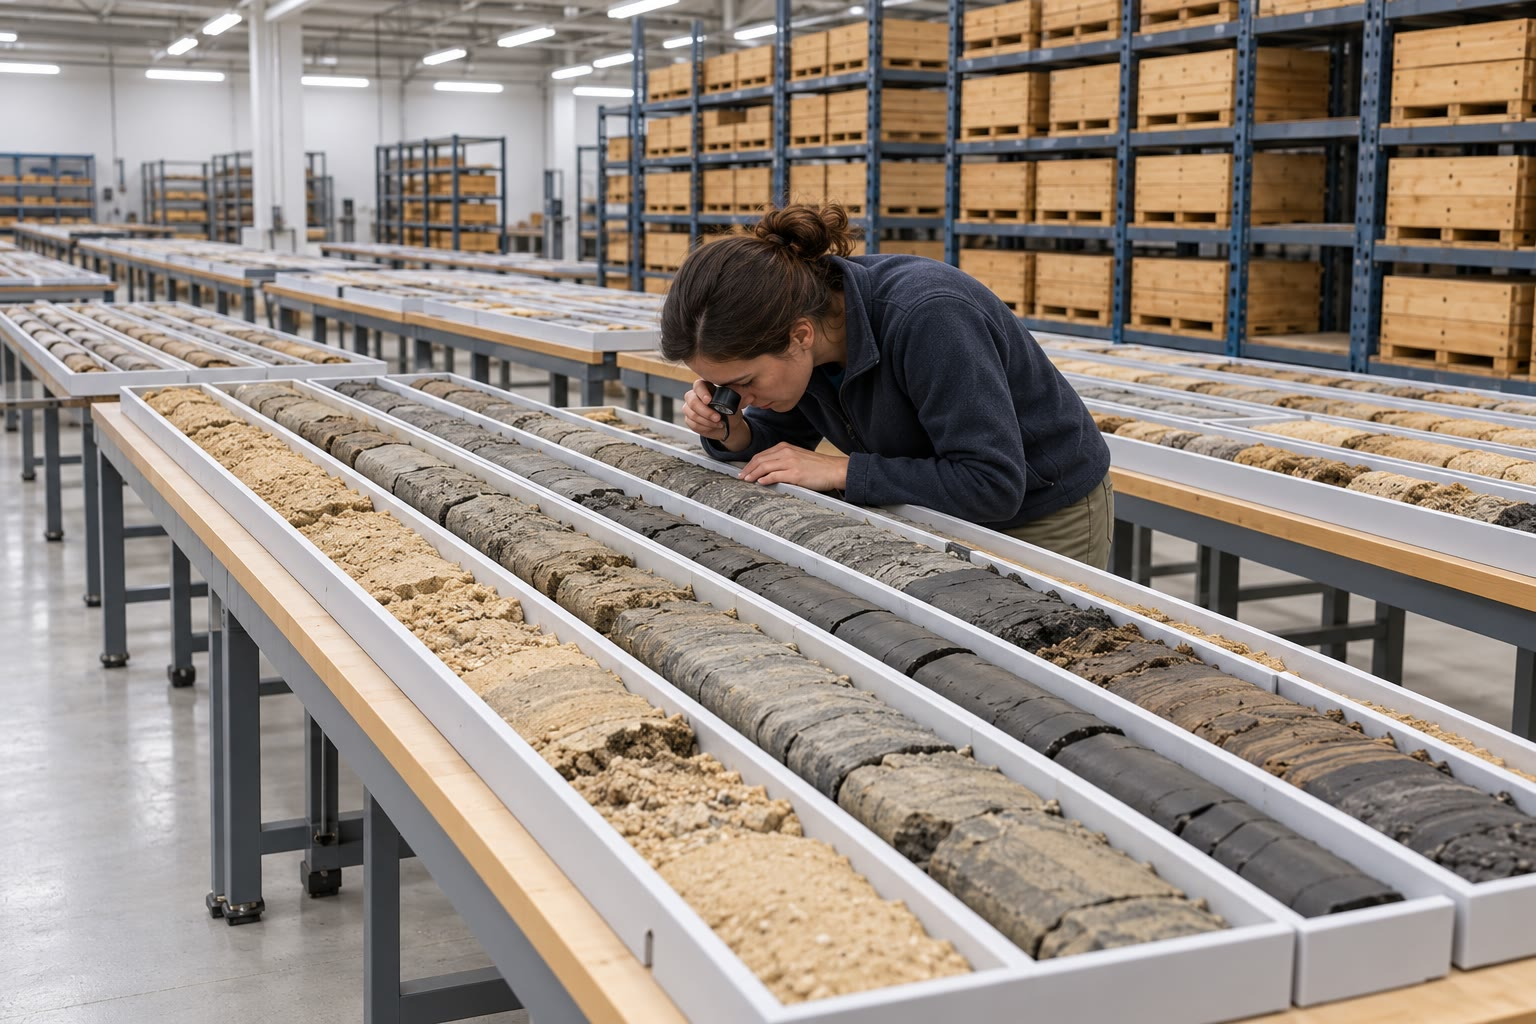
\includegraphics[width=\linewidth]{images/book5/ai/b3-core-store.jpg}

{\scriptsize A core store: split cores of sand and mud in trays, a geologist
with a hand lens. AI-generated illustration.}
\end{minipage}
\end{inthelab}

\section{Exercises}

\begin{exercise}[$\star$]\label{exo:b3:facies-models:1}
A core shows, from the base up: offshore mud, interbedded mud and fine sand,
\omterm{def:b3:facies-models:shoreface}{shoreface} sand, beach sand, then coal with roots. Using Walther's law, give
the order of the environments along the coast at the time and the direction
in which the shoreline moved. What would a transgression have left?
\end{exercise}

\begin{exercise}[$\star$]\label{exo:b3:facies-models:2}
Three sand bodies show gamma-ray shapes: (a) a bell \qty{8}{m} thick with a
sharp base; (b) a funnel \qty{20}{m} thick; (c) a cylinder \qty{30}{m}
thick with sharp top and base. Suggest an environment for each, and the
observation in a core that would confirm it.
\end{exercise}

\begin{exercise}[$\star$]\label{exo:b3:facies-models:3}
A sandstone reads $\rho_b = \qty{2.40}{g/cm^3}$. Compute its porosity with a
quartz matrix and fresh water, then with brine of \qty{1.1}{g/cm^3}.
\end{exercise}
% ledger: keys:density-porosity

\begin{exercise}[$\star$]\label{exo:b3:facies-models:4}
Waves of modal wavelength \qty{75}{m} and \qty{110}{m} (the sheltered and
the open seas of the buoy study). Estimate the depth at which each keeps
\qty{4}{\percent} of its surface motion, and the fraction left at a depth of
\qty{20}{m}.
\end{exercise}
% ledger: losspeters10:wavebase

\begin{exercise}[$\star\star$]\label{exo:b3:facies-models:5}
A limestone reads $\Delta t = \qty{60}{\micro\second/ft}$. Compute its
porosity with the time-average equation for a matrix of 47.6 and of
\qty{52.6}{\micro\second/ft} and brine at \qty{189}{\micro\second/ft}. What
does the difference teach?
\end{exercise}
% ledger: keys:sonic

\begin{exercise}[$\star\star$]\label{exo:b3:facies-models:6}
A \qty{40}{m} interval holds sand beds of 6.0, 3.5, 8.0 and \qty{2.5}{m}
below the cutoff, the rest mud. Compute its \omterm{def:b3:facies-models:ntg}{net-to-gross ratio}. With a
porosity of \qty{22}{\percent} in the sand, how much pore volume does a
square kilometre of the interval hold?
\end{exercise}

\begin{exercise}[$\star\star$]\label{exo:b3:facies-models:7}
A turbidite bed near the mouth of a canyon is \qty{1.2}{m} of massive sand
(Ta) eroded at the top by the next bed; \qty{30}{km} down the fan a bed of
the same flow is \qty{8}{cm} of ripple-laminated fine sand and silt under
\qty{3}{cm} of mud. Name the divisions of each and explain the change.
\end{exercise}

\begin{exercise}[$\star\star$]\label{exo:b3:facies-models:8}
A \omterm{def:b3:facies-models:association}{fining-upward succession} \qty{9}{m} thick has a sharp base with pebbles,
cross-bedded sand, rippled fine sand and rooted mud. Interpret it, and
estimate the depth of the channel that built it. Can Walther's law be
applied across its base? Why?
\end{exercise}

\begin{exercise}[$\star\star$]\label{exo:b3:facies-models:9}
A platform floor drops \qty{60}{m} over \qty{40}{km}; another keeps a
depth of \qty{5}{m} for \qty{30}{km}, then drops \qty{300}{m} over
\qty{1.5}{km}. Compute both gradients, name each platform and the facies
expected at the edge of the second.
\end{exercise}

\begin{exercise}[$\star\star\star$]\label{exo:b3:facies-models:10}
A shoreline progrades at a speed $v$ while relative sea level rises at a rate
$A$, and its \omterm{def:b3:facies-models:shoreface}{shoreface} belt is $w$ wide. Show that the \omterm{def:b3:facies-models:shoreface}{shoreface} sand in the
vertical succession is $h = wA/v$ thick. Compute it for $w = \qty{2}{km}$,
$A = \qty{0.2}{m/kyr}$ and $v = \qty{20}{m/kyr}$, and say what happens when
$A = 0$. Compare with the proposition on the \omterm{def:b3:sequence-stratigraphy:trajectory}{shoreline trajectory} of
Chapter~\ref{ch:b3:sequence-stratigraphy}.
\end{exercise}

\begin{exercise}[$\star\star\star$]\label{exo:b3:facies-models:11}
A sandstone reads $\rho_b = \qty{2.30}{g/cm^3}$ and $\Delta t =
\qty{86}{\micro\second/ft}$. Compute its porosity from each log with a quartz
sandstone matrix (2.65, \qty{52.6}{\micro\second/ft}) and brine (1.0 for the
density, \qty{189}{\micro\second/ft}). If the sonic porosity is right, what
grain density does the \omterm{def:b3:facies-models:wireline}{density log} imply, and what may the cement be?
\end{exercise}
% ledger: keys:density-porosity, keys:sonic

\begin{exercise}[$\star\star\star$]\label{exo:b3:facies-models:12}
In a core, black offshore mud rests directly on a coal with roots, with a
thin layer of shell debris at the contact. Explain why Walther's law does
not apply across it, what surface it is, and how much of the coastal
succession may be missing if waves eroded the floor down to a \omterm{def:b3:facies-models:shoreface}{fair-weather
wave base} of about \qty{10}{m} as the shoreline passed.
\end{exercise}

\section{Problem: Varden-2, a Well through the Cover}

\begin{problem}[{Weekend problem --- the logs, porosity, facies and net sand
of an invented well in the Varden syncline}]
\label{pb:b3:facies-models:1}
The well Varden-2 is drilled in the syncline of the Varden Hills, at
(7500, 7000) on the region's grid, from a ground elevation of
\qty{441.0}{m}, to a total depth of \qty{1200}{m}. Its logs are drawn in the
figure of the last section. Use grain densities of 2.65 (quartz) and
\qty{2.71}{g/cm^3} (calcite), a pore water of \qty{1.0}{g/cm^3}, matrix
transit times of 52.6 (sandstone) and \qty{47.6}{\micro\second/ft}
(limestone), and \qty{189}{\micro\second/ft} for the water.

\medskip\noindent\textbf{Part I --- Reading the logs.}
\begin{enumerate}
\item The gamma ray jumps from 12 to \qty{110}{API} at \qty{766}{m}, falls
  to 18 at \qty{866}{m}, becomes irregular from \qty{1046}{m} and steady at
  \qty{85}{API} from \qty{1166}{m}. Name the units met, using their logs.
\item Compute the thickness of each unit of the cover and the elevation of
  the base of the cover.
\item The chalk reads \qty{2.03}{g/cm^3} near the surface and
  \qty{2.36}{g/cm^3} at \qty{750}{m}. Compute its porosity at both depths.
  What happens to the chalk with depth?
\item Why is the shale not given a porosity from its density?
\item The schist reads \qty{2.75}{g/cm^3} and \qty{50}{\micro\second/ft}.
  What does the fast, dense, non-porous basement tell the driller?
\end{enumerate}

\medskip\noindent\textbf{Part II --- Porosity.}
\begin{enumerate}[resume]
\item The limestone reads \qty{2.573}{g/cm^3}: compute its density porosity.
\item It reads \qty{58.9}{\micro\second/ft}: compute its sonic porosity and
  compare.
\item The clean sand of the channel fills reads \qty{2.32}{g/cm^3}: compute
  its porosity.
\item Check it with its transit time, \qty{79.9}{\micro\second/ft}.
\item If the pore water were a brine of \qty{1.1}{g/cm^3}, by how much would
  the density porosity of the sand change?
\item Which unit would make the better aquifer or reservoir, and which the
  seal above it?
\end{enumerate}

\medskip\noindent\textbf{Part III --- Facies.} A core cut from 1108 to
\qty{1124}{m} shows, from the base: a scoured surface with mud clasts and
pebbles; \qty{10.4}{m} of cross-bedded medium sand; \qty{3.2}{m} of rippled
fine sand passing into silt; \qty{2.4}{m} of red-brown mud with root traces.
\begin{enumerate}[resume]
\item Draw the gamma-ray shape expected through the cored interval.
\item Name the succession and the environment of each part.
\item With Walther's law, describe the environments that lay side by side.
\item Estimate the depth of the channel.
\item The sandstone holds eleven such units, each on a sharp base. What does
  the stacking tell about the river and its plain?
\item Can Walther's law be used to go from one unit to the next? Why?
\end{enumerate}

\medskip\noindent\textbf{Part IV --- Net sand.} The eleven channel fills,
from the base of the sandstone, are 14, 9, 12, 7, 16, 10, 13, 8, 11, 12 and
\qty{8}{m} thick. Each starts with clean sand (\qty{30}{API}) over a share
of its thickness of 0.60, 0.45, 0.55, 0.30, 0.65, 0.40, 0.55, 0.35, 0.50,
0.45 and 0.30, then fines upward over a share of 0.25, 0.30, 0.25, 0.40,
0.20, 0.30, 0.25, 0.35, 0.25, 0.30 and 0.35, the gamma ray rising linearly to
\qty{105}{API}, and ends in mud.
\begin{enumerate}[resume]
\item Which fraction of each fining interval lies below the \qty{60}{API}
  cutoff?
\item Compute the net sand of the lowest unit and of the thickest.
\item Compute the clean-sand total and the fining-interval total of the
  sandstone.
\item Compute its \omterm{def:b3:facies-models:ntg}{net-to-gross ratio}.
\item How would the net sand change with a cutoff of 45 or of
  \qty{75}{API}?
\item With the sand porosity of question 8, compute the pore volume of the
  net sand under a square kilometre.
\item State the net sand thickness of the Triassic sandstone at Varden-2.
\end{enumerate}
\end{problem}
% ledger: keys:density-porosity, keys:sonic, keys:gamma
